\documentclass[tikz,border=5pt]{standalone}
\usepackage{amsmath,amssymb}
\usetikzlibrary{arrows.meta}
\definecolor{curveblue}{HTML}{245C86}
\definecolor{accent}{HTML}{A65E2E}
\begin{document}
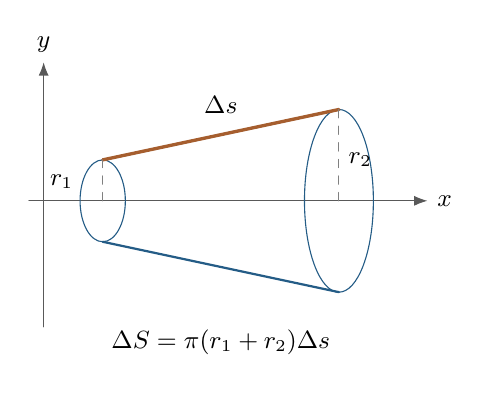
\begin{tikzpicture}[font=\small,>=Latex,line cap=round,line join=round]
\begin{scope}[shift={(0.00000,0.00000)},xscale=1.25,yscale=0.8]
\draw[->,black!65] (-0.15000,0.00000)--(3.90000,0.00000);
\node[right] at (3.90000,0.00000) {$x$};
\draw[->,black!65] (0.00000,-2.00000)--(0.00000,2.20000);
\node[above] at (0.00000,2.20000) {$y$};
\draw[curveblue,thick] (0.60000,-0.65000)--(3.00000,-1.45000);
\draw[curveblue,thick] (0.60000,0.65000)--(3.00000,1.45000);
\draw[curveblue] (.6,0) ellipse (.23 and .65);\draw[curveblue] (3,0) ellipse (.35 and 1.45);\draw[accent,very thick] (0.60000,0.65000)--(3.00000,1.45000);
\node[above] at (1.80000,1.23000) {$\Delta s$};
\draw[gray,dashed] (0.60000,0.00000)--(0.60000,0.65000);
\node[left] at (0.40000,0.30000) {$r_1$};
\draw[gray,dashed] (3.00000,0.00000)--(3.00000,1.45000);
\node[right] at (3.00000,0.65000) {$r_2$};
\node[below] at (1.80000,-1.90000) {$\Delta S=\pi(r_1+r_2)\Delta s$};
\end{scope}
\end{tikzpicture}
\end{document}
